\begin{figure*}[t]
    \centering
    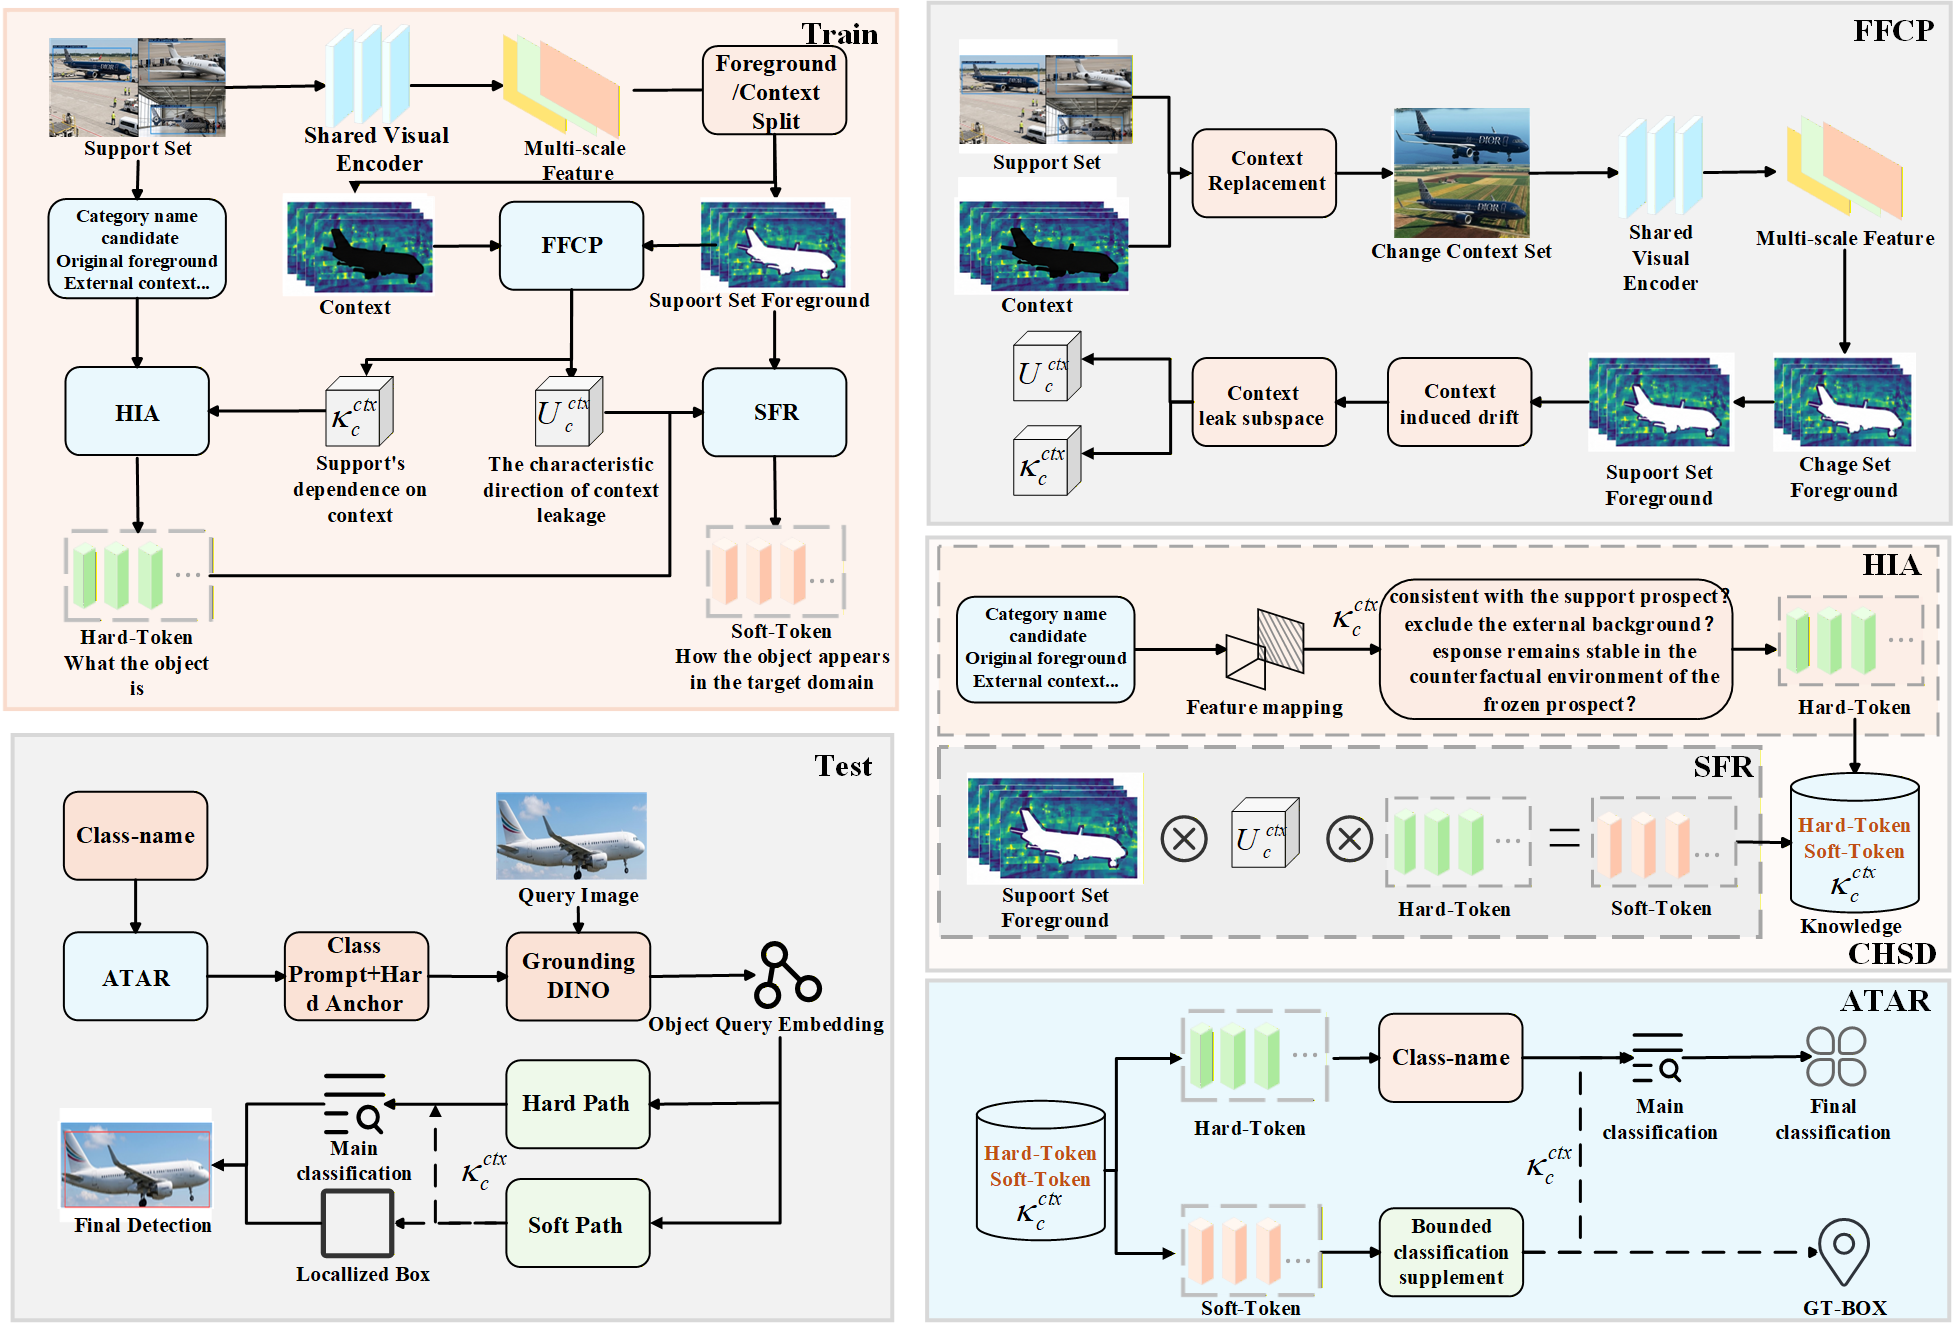
\includegraphics[width=\textwidth]{fig/method_overview.png}
    \caption{\textbf{Knowledge-enhanced Hard--Soft framework.} (1) Foreground-Frozen Context Probing (FFCP) modifies only the support context and estimates a class-wise context-sensitive subspace. (2) Context-Constrained Hard--Soft Decomposition (CHSD) builds a bounded Hard identity anchor and a context-cleaned Soft appearance residual. (3) Grounding DINO first produces its ordinary query predictions. (4) Asymmetric Task-Authority Routing (ATAR) uses Hard--Soft agreement and baseline-query uncertainty to authorize a bounded cosine class correction while leaving the localization output unchanged.}
    \label{fig:overview}
\end{figure*}
